\section{Results}

The results in this chapter are entirely based on the test set, which had no contact with the network up to this point. It was also made sure that there was no overlap in images of people that were recorded multiple times. 5 images were chosen randomly from each of the two sources in the very beginning. Since the Epi data featured 41 slices and the Jopp data featured 24 slices, 325 2D samples were available for evaluation. Each slice contained 50,176 pixel values, making a total of 16.3 million predictions that were analyzed.

The network architecture was developed and optimized with focus on a single segmentation channel that merged Femur, Tibia und Fibula maps. However, tests were also run to validate the performance for each bone on its own. The same architecture and training procedure was used for this task.

\subsection{Numeric Evaluation}

The proposed model achieves a DICE score of 98.0\% and an IoU of 96.0\%. Precision and Recall are perfectly balanced at 98.0\% as well, suggesting that predictions are neither too optimistic or pessimistic. The error shows a small value of 1.2\% when looking at falsely predicted areas in relationship to the entire frame.

\begin{table}[H]
    \centering
    \begin{tabular}{| l | c | c | c | c | c |}
    \hline
           & DSC & IoU & Precision & Recall & Error \\ 
    \hline
    Merged   & \makecell{0.980} 
             & \makecell{0.960} 
             & \makecell{0.980} 
             & \makecell{0.980} 
             & \makecell{0.012} \\
    \hline
    Femur    & \makecell{0.981} 
             & \makecell{0.963} 
             & \makecell{0.979} 
             & \makecell{0.984} 
             & \makecell{0.006} \\
    \hline
    Tibia    & \makecell{0.977} 
             & \makecell{0.955} 
             & \makecell{0.976} 
             & \makecell{0.977} 
             & \makecell{0.006} \\
    \hline
    Fibula   & \makecell{0.953} 
             & \makecell{0.911} 
             & \makecell{0.954} 
             & \makecell{0.952} 
             & \makecell{0.001} \\
    \hline
    Combined & \makecell{0.979} 
             & \makecell{0.958} 
             & \makecell{0.977} 
             & \makecell{0.981} 
             & \makecell{0.004} \\
    \hline
    \end{tabular}
    \caption{Numeric evaluation of the test set using popular metrics}
\end{table}

Results on Femur and Tibia alone are comparable to the merged approach, whereas the Fibula segmentation reaches a DSC of 95.3\% and IoU of 91.1\%. This could be due to the fact that the Fibula is only visible in a minority of slices, making it a fairly unbalanced task. Combining the three separate segmentations to a single model gives comparable results as well. The error is even reduced by a factor of 3, which is expected because the segmentation channels are also increased by 3.

A study from 2011 ran a similar segmentation on the knee \cite{Martel-Pelletier2011}, achieving a DSC of 94\% for the femur and 92\% for the tibia using the ray casting technique. Another study from 2015 \cite{Dam} used an atlas based segmentation and achieved a DSC of 97.5\% for the tibia.

\subsection{Visual Evaluation}

The visual evaluation will focus on the results of the combined network since its performance is on par with the one channel model while offering more information about the associated bones.

\begin{figure}[H]
\centering
\par
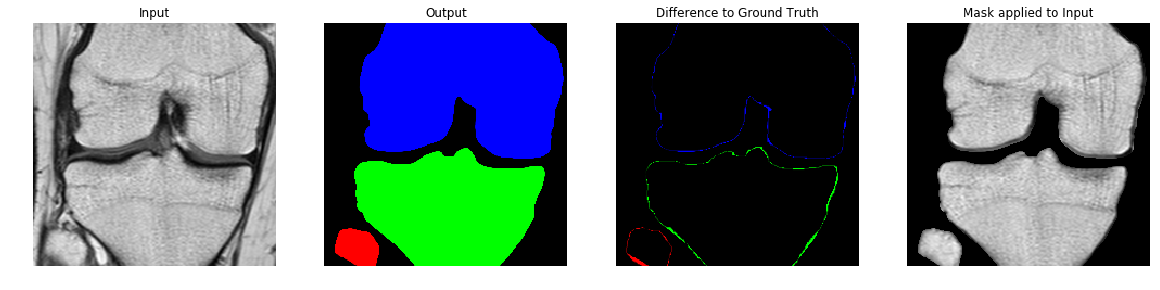
\includegraphics[width=1.0\textwidth]{imgs/sample1.png}
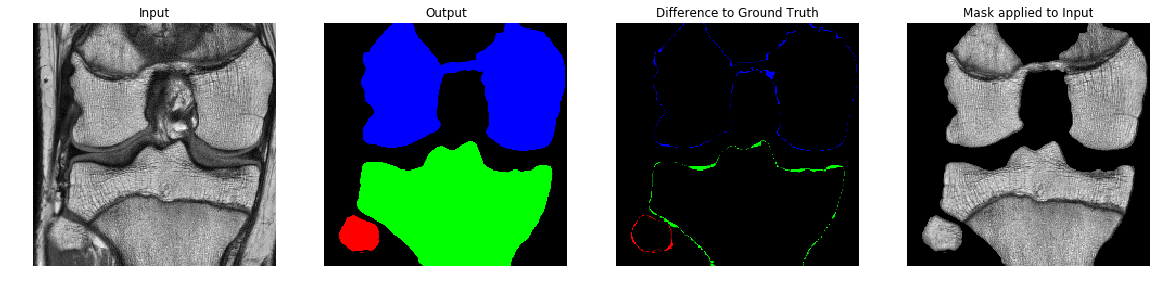
\includegraphics[width=1.0\textwidth]{imgs/sample2.png}
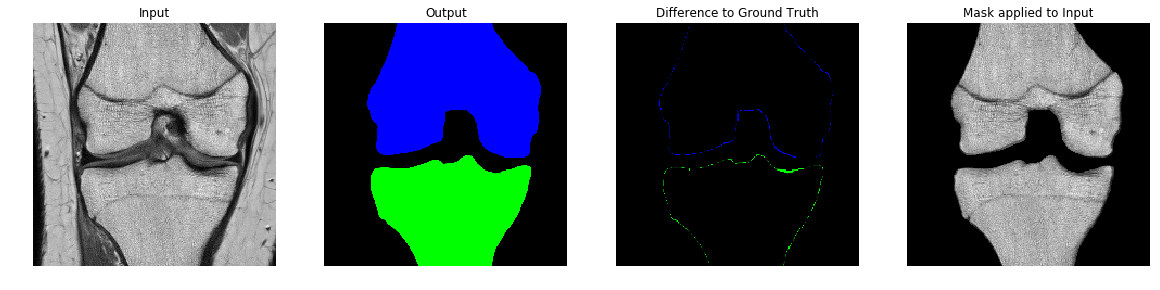
\includegraphics[width=1.0\textwidth]{imgs/sample4.png}
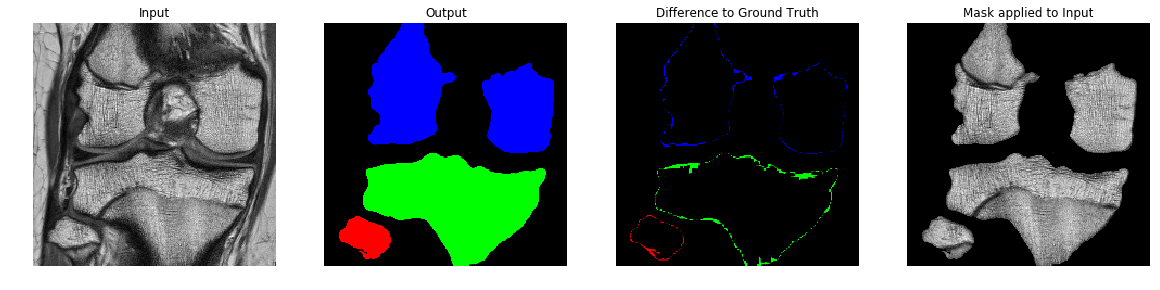
\includegraphics[width=1.0\textwidth]{imgs/sample3.png}
\caption{Input, predicted output, difference to ground truth and mask applied on input}
\par
\end{figure}

The network shows excellent performance on slices that are located near the middle of the 3D MRIs with DSC scores of over 99\%

\begin{figure}[H]
\centering
\par
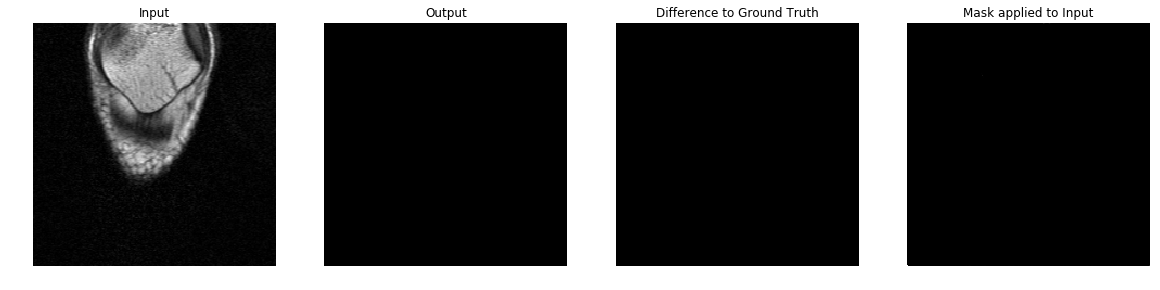
\includegraphics[width=1.0\textwidth]{imgs/sample5.png}
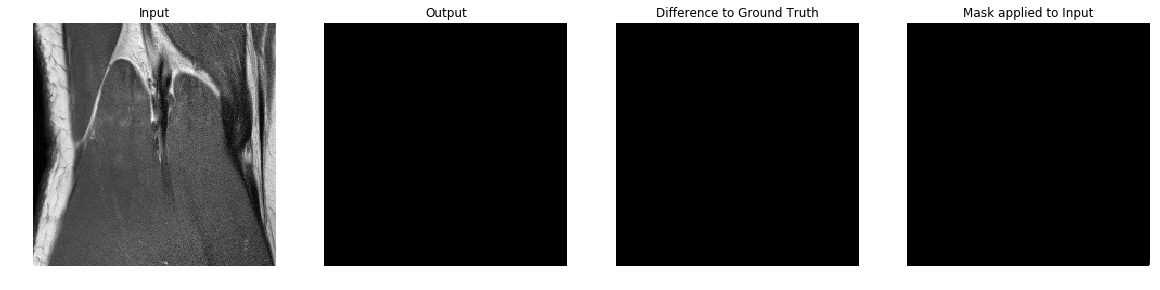
\includegraphics[width=1.0\textwidth]{imgs/sample6.png}
\caption{Input, predicted output, difference to ground truth and mask applied on input}
\par
\end{figure}

The best DSC scores of 100\% are achieved through empty segmentations that the network correctly predicted as such.

\begin{figure}[H]
\centering
\par
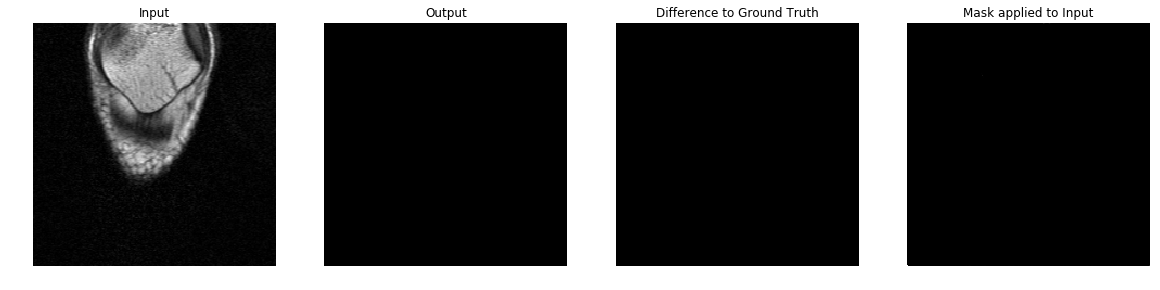
\includegraphics[width=1.0\textwidth]{imgs/sample5.png}
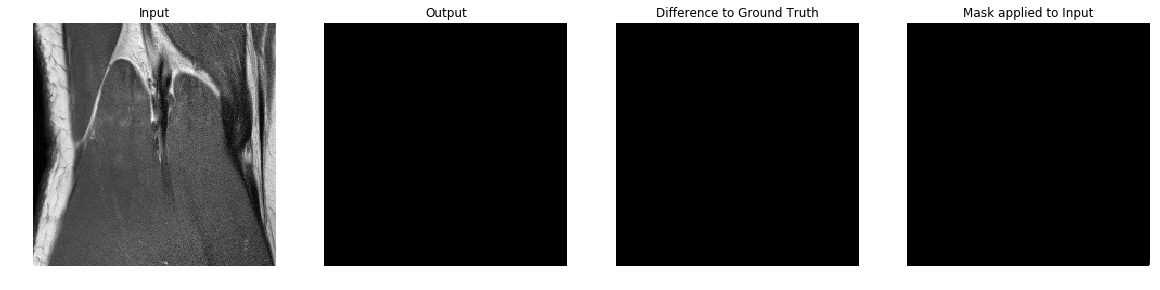
\includegraphics[width=1.0\textwidth]{imgs/sample6.png}
\caption{Input, predicted output, difference to ground truth and mask applied on input}
\par
\end{figure}

The worst results appeared in upper and lower slices where the bones started to become visible. Oftentimes the network didn't agree with the ground truth on what could already be interpreted as bone. If either the prediction or the ground truth was empty while the other was not 

If the ground truth was empty and the prediction was not resulted in a DSC of 0\%

\subsection{Transfer Experiments}

Neural networks are known to be unreliable when used on data that exceeds the range of variation in the training set. Then again, convolutions are translation invariant, allowing them to recognize patterns anywhere in the frame \cite{Chollet2017}. Another merged model was trained that used the same architecture but added further image augmentation of horizontal and vertical flips. This way it only reached a DSC score of 97.3\% but was more flexible to structural differences in the image.

\subsubsection{Resolution Variance}

The proposed architecture can be described as "fully convolutional" because it doesn't include any dense layers. This allows the network to accept any kind of resolution and still being able to process it. An experiment was set up that used uncropped Epi image resized to 448x448 making them 4 times larger.

\begin{figure}[H]
\minipage{0.24\textwidth}
  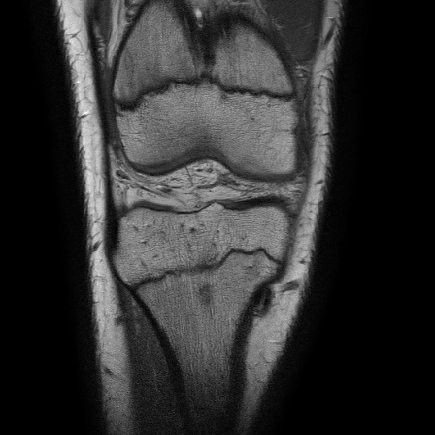
\includegraphics[width=\linewidth]{imgs/transfer_size_x1.png}
\endminipage\hfill
\minipage{0.24\textwidth}
  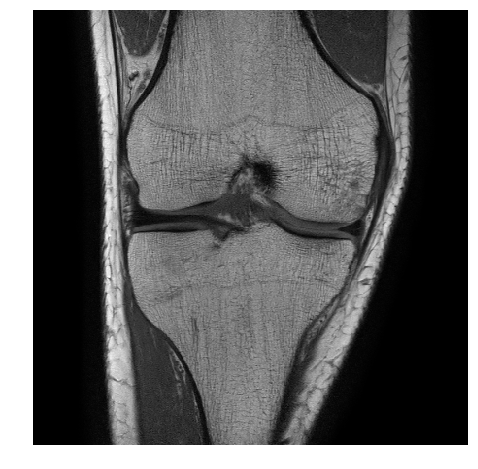
\includegraphics[width=\linewidth]{imgs/transfer_size_x2.png}
\endminipage\hfill
\minipage{0.24\textwidth}%
  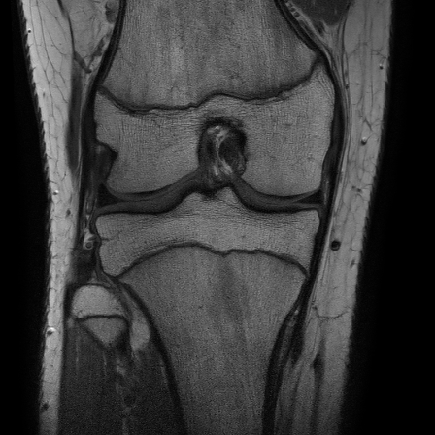
\includegraphics[width=\linewidth]{imgs/transfer_size_x3.png}
\endminipage\hfill
\minipage{0.24\textwidth}%
  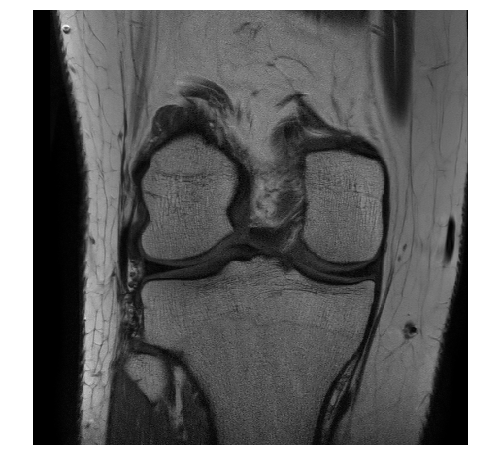
\includegraphics[width=\linewidth]{imgs/transfer_size_x4.png}
\endminipage
\vspace{0.15cm}
\minipage{0.24\textwidth}
  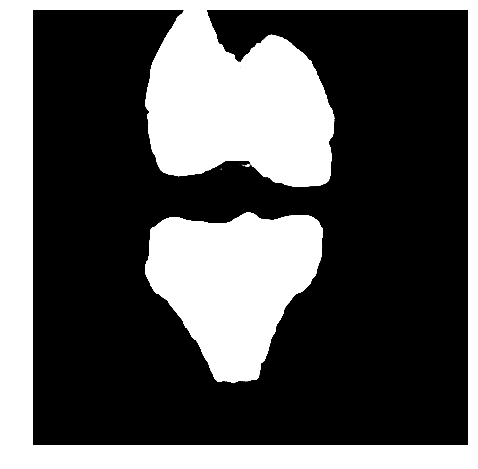
\includegraphics[width=\linewidth]{imgs/transfer_size_y1.png}
\endminipage\hfill
\minipage{0.24\textwidth}
  
\includegraphics[width=\linewidth]{imgs/transfer_size_y2.png}
\endminipage\hfill
\minipage{0.24\textwidth}%
  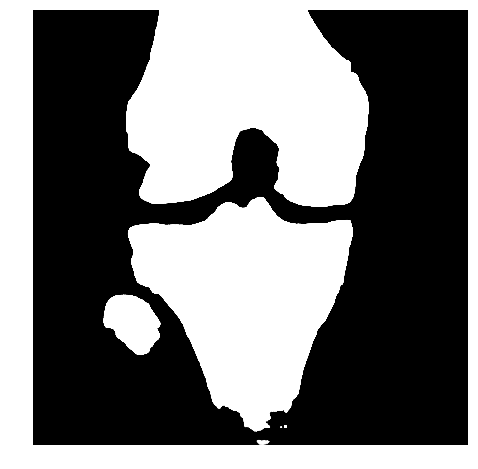
\includegraphics[width=\linewidth]{imgs/transfer_size_y3.png}
\endminipage\hfill
\minipage{0.24\textwidth}%
  
\includegraphics[width=\linewidth]{imgs/transfer_size_y4.png}
\endminipage
\caption{Four random samples uncropped of Epi data segmentations that were resized to 448x448 pixels}
\end{figure}

The predictions look surprisingly good even following the shaft of the bone which wasn't visible in the cropped versions it was trained on. Even large intensity gaps through growth plates are recognized as Femur or Tibia. The recall performance is very accurate based on a subjective visual evaluation of random samples. Problems are visible in tissue that isn't bone but was recognized as such like in the fourth sample image.

\subsubsection{Perspective Variance}

In 3.2 a third data source was mentioned that featured 5 sagittal recordings of knees. These were not used for the training because of their structural differences. The following samples show what happens when the network is applied to images from a different perspective.

\begin{figure}[H]
\minipage{0.24\textwidth}
  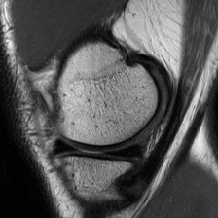
\includegraphics[width=\linewidth]{imgs/transfer_pers_x1.png}
\endminipage\hfill
\minipage{0.24\textwidth}
  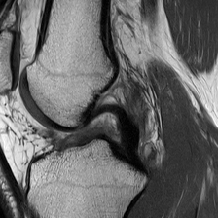
\includegraphics[width=\linewidth]{imgs/transfer_pers_x2.png}
\endminipage\hfill
\minipage{0.24\textwidth}%
  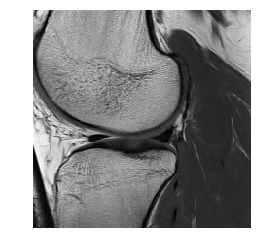
\includegraphics[width=\linewidth]{imgs/transfer_pers_x3.png}
\endminipage\hfill
\minipage{0.24\textwidth}%
  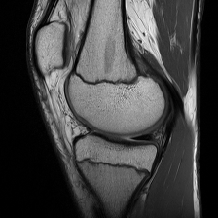
\includegraphics[width=\linewidth]{imgs/transfer_pers_x4.png}
\endminipage
\vspace{0.15cm}
\minipage{0.24\textwidth}
  
\includegraphics[width=\linewidth]{imgs/transfer_pers_y1.png}
\endminipage\hfill
\minipage{0.24\textwidth}
  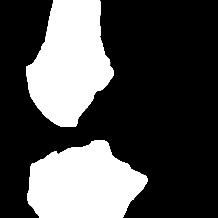
\includegraphics[width=\linewidth]{imgs/transfer_pers_y2.png}
\endminipage\hfill
\minipage{0.24\textwidth}%
  
\includegraphics[width=\linewidth]{imgs/transfer_pers_y3.png}
\endminipage\hfill
\minipage{0.24\textwidth}%
  
\includegraphics[width=\linewidth]{imgs/transfer_pers_y4.png}
\endminipage
\caption{Four random samples of sagittal Maas data segmentations using the coronal trained model}
\end{figure}

Subjectively, these results look excellent. In example 4 it even recognizes the Patella, a bone it was never trained on. This shows that with enough image augmentation the network will learn to segment any type of bone.

\subsection{Age Prediction}

The initial cause for the segmentation experiment was to reduce the amount of information in a knee MRI. The resulting images could then be used to make age related predictions that focussed on the bone and the growth plate. This section will briefly cover such an age prediction pipeline.

The age of the candidates ranged from 14 to 21 years with a mean at 17.5 years. Predicting this age for every person meant that it was never off more than 3.5 years. Since the data was normally distributed, a static prediction of the mean led to a mean absolute error (MAE) of 1.2 years.

Even by using many of the techniques mentioned in previous chapters, I was not able to train a stable model that could beat this baseline on the raw input data. After the segmentation maps were applied to all 145 3D samples many of the slices were completely empty because they didn't contain any of the three bones. It was decided to only use the middle 18 slices from each of the two sources. Out of these resulting 2610 slices 2124 were used for the training set, but the network still wouldn't converge.

Only after using the contracting side of the proposed model with the parameters it learned on the segmentation task was I able to train a network in a stable manner. This approach did not make the model converge every time, but when it did its predictions were stable through multiple epochs. 

The results on the test data showed a MAE of 0.61 years for all of the slices. Since every 3D sample now had 18 different predictions, I build another tree based model that would take a vector of 18 values and predict a single age. This got a final MAE of 0.54 years on the test data, which is more than twice as good as the already competitive baseline.

\newpage